\section{Support Vector Machines (SVM)}
Support Vector Machines were first introduced by Vapnik and Chervonenkis in \cite{VC74}. The core idea is to find the optimal hyperplane to seperate a dataset, while there are theoretically infinite hyperplanes to seperate the dataset. A hyperplane is chosen, so that the distance to the nearest datapoint of both classes is maximized (Figure \ref{fig:maximum_margin}). The points spanning the hyperplane are the \textit{Support Vectors}, hence the name \textit{Support Vector Machines}. \cite{VC95}

\begin{figure}
\begin{center}
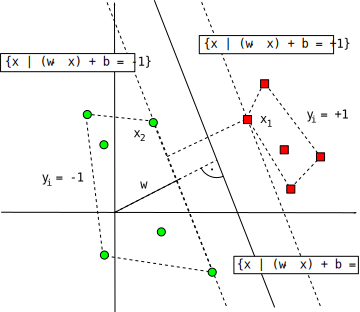
\includegraphics[scale=0.7]{img/svm/margin.pdf}
 % margin.pdf: 289x250 pixel, 72dpi, 10.20x8.82 cm, bb=0 0 289 250
\end{center}
 \caption{Maxmimum Margin Classifier.}
 \label{fig:maximum_margin}
\end{figure}

\subsection{Definition}
Given a Set of Datapoints $\mathcal{D}$:

$$\mathcal{D} = \left\{(x_i, y_i) | x_i \in \mathbb{R}^p, y_i \in \left\{-1,1\right\}\right\}_{i=1}^n$$
where
\begin{itemize}
 \item $x_i$ is a point in p-dimensional vector
 \item $y_i$ is the corresponding class label
\end{itemize}
We search for $\omega \in \mathbb{R}^n$ and bias $b$, forming the Hyperplane H:
$$\omega^T x + b = 0$$
that seperates both classes so that:
$$ \omega^T x + b = 1,\mbox{if } y = 1 $$
$$ \omega^T x + b = -1, \mbox{if } y = -1 $$

The optimization problem that needs to be solved is:
$$\mbox{min } \frac{1}{2}\omega^T \omega$$
subject to:
$$\omega^T x + b \geq 1, y = 1$$
$$\omega^T x + b \leq 1, y = -1 $$

Such quadratic optimization problems can be solved with standard solvers, such as \htmladdnormallink{GNU Octave}{www.gnu.org/software/octave} or \htmladdnormallink{Matlab}{www.mathworks.com/products/matlab}.

\subsubsection{Non-linear SVM}
The kernel trick is used for classifying non-linear datasets. It works by transforming data points into a higher dimensional feature space with a \textit{kernel function}, where the dataset can be seperated again (see Figure \ref{fig:kernel_trick}).


\begin{figure}[ht!]
\begin{center}
 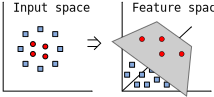
\includegraphics[scale=1.3]{img/svm/input_space2.pdf}
 \caption{Kernel Trick}
 \label{fig:kernel_trick}
 % input_space2.pdf: 1179666x1179666 pixel, 0dpi, infxinf cm, bb=
\end{center}
\end{figure}


Commonly used kernel functions are \textit{RBF kernels}:
$$k(x,x') = exp(\frac{\|x-x'\|^2}{\sigma^2})$$ 
or \textit{polynomial kernels}:
$$k(x,x') = (x \cdot x')^d$$.



\subsection{SVM in OpenCV}
Parameters for a SVM have to be defined in the structure \textit{CvSVMParams}.

\subsubsection*{Parameters}
\begin{lstlisting}[language=C++, caption=Example CvSVMParams, label=lst:cvsvmparams]
CvSVMParams param = CvSVMParams();

param.svm_type = CvSVM::C_SVC;
param.kernel_type = CvSVM::LINEAR;

param.degree = 0; // for poly
param.gamma = 20; // for poly/rbf/sigmoid
param.coef0 = 0; // for poly/sigmoid

param.C = 7; // for CV_SVM_C_SVC, CV_SVM_EPS_SVR and CV_SVM_NU_SVR
param.nu = 0.0; // for CV_SVM_NU_SVC, CV_SVM_ONE_CLASS, and CV_SVM_NU_SVR
param.p = 0.0; // for CV_SVM_EPS_SVR

param.class_weights = NULL; // for CV_SVM_C_SVC
param.term_crit.type = CV_TERMCRIT_ITER | CV_TERMCRIT_EPS;
param.term_crit.max_iter = 1000;
param.term_crit.epsilon = 1e-6;
\end{lstlisting}
Where the parameters are (taken from the OpenCV documentation):
\begin{itemize}
 \item \lstinline|svm_type|
 \begin{itemize}
  \item \lstinline|CvSVM::C_SVC| n-class classification ($n \geq 2$), allows imperfect separation of classes with penalty multiplier C for outliers.
  \item \lstinline|CvSVM::NU_SVC| n-class classification with possible imperfect separation. Parameter nu (in the range $0\ldots1$, the larger the value, the smoother the decision boundary) is used instead of C.
  \item \lstinline|CvSVM::ONE_CLASS| one-class SVM. All the training data are from the same class, SVM builds a boundary that separates the class from the rest of the feature space.
  \item \lstinline|CvSVM::EPS_SVR| regression. The distance between feature vectors from the training set and the fitting hyper-plane must be less than p. For outliers the penalty multiplier C is used.
  \item \lstinline|CvSVM::NU_SVR| regression; nu is used instead of p. 
 \end{itemize}
\item \lstinline|kernel_type|
\begin{itemize}
 \item \lstinline|CvSVM::LINEAR| no mapping is done, linear discrimination (or regression) is done in the original feature space. It is the fastest option. $d(x,y) = x \cdot y == (x,y)$.
 \item \lstinline|CvSVM::POLY| polynomial kernel: $d(x,y) = (gamma * (x \cdot y) + coef0)^{degree}$.
 \item \lstinline|CvSVM::RBF| radial-basis-function kernel; a good choice in most cases: $d(x,y) = exp(-gamma*|x-y|^2)$.
 \item \lstinline|CvSVM::SIGMOID| sigmoid function is used as a kernel: $d(x,y) = tanh(gamma * (x \cdot y) + coef0)$.
\end{itemize}
 \item \lstinline|C, nu, p| Parameters in the generalized SVM optimization problem. 
\item \lstinline|class_weights| Optional weights, assigned to particular classes. They are multiplied by C and thus affect the misclassification penalty for different classes. The larger weight, the larger penalty on misclassification of data from the corresponding class.
\item \lstinline|term_criteria| Termination procedure for iterative SVM training procedure (which solves a partial case of constrained quadratic optimization problem)
 \begin{itemize}
  \item \lstinline|type| is either \lstinline|CV_TERMCRIT_ITER| or \lstinline|CV_TERMCRIT_ITER| 
  \item \lstinline|max_iter| is the maximum number of iterations in training.
  \item \lstinline|epsilon| is the error to stop training.
 \end{itemize}
\end{itemize}

\subsubsection*{Training}
Training can either be done by passing the vector with the training data and vector with the corresponding class labels to the constructor or the train method.
\begin{lstlisting}[language=C++]
CvSVM(const CvMat* _train_data, 
      const CvMat* _responses,
      const CvMat* _var_idx=0,
      const CvMat* _sample_idx=0,
      CvSVMParams _params=CvSVMParams());
\end{lstlisting}
where
\begin{itemize}
 \item \textbf{\_train\_data} is a Matrix with the n-dimensional feature vectors
 \item \textbf{\_responses} is a vector with the class for the corresponding feature vector
 \item \textbf{\_var\_idx} identifies features of interest (can be left empty for this example, in code: \texttt{cv::Mat()})
 \item \textbf{\_sample\_idx} identifies samples of interest (can be left empty for this example, in code: \texttt{cv::Mat()})
 \item \textbf{\_params} Parameter for the SVM from Listing \ref{lst:cvsvmparams}
\end{itemize}
This applies to the train method aswell:
\begin{lstlisting}[language=C++]
virtual bool train(const CvMat* _train_data, 
  const CvMat* _responses,
  const CvMat* _var_idx=0,
  const CvMat* _sample_idx=0,
  CvSVMParams _params=CvSVMParams() );
\end{lstlisting}

The \textit{train} methods of the SVM has some limitations (at time of writing this):

 \begin{itemize}
  \item Only \verb|CV_ROW_SAMPLE| is supported
  \item Missing measurements are not supported
 \end{itemize}
The \textit{train\_auto} method finds the best parameters with a Gridsearch and a k-fold cross validation. This method is available for OpenCV Versions $\geq$ 2.0.

\subsubsection*{Prediction}
Self explaining code.
\begin{lstlisting}[language=C++]
for(int i = 0; i < testData.rows; i++) {
	cv::Mat sample = testData.row(i);
	float result = svm.predict(sample);
}
\end{lstlisting}

\subsubsection*{Support Vectors}
The support vectors of a SVM can be obtained using the \lstinline|get_support_vector| function of the API:
\begin{lstlisting}[language=C++]
int svec_count = svm.get_support_vector_count();
for(int vecNum = 0; vecNum < svec_count; vecNum++) {
	const float* vec = svm.get_support_vector(vecNum);
}
\end{lstlisting}


A complete example for Support Vector Machines in OpenCV is given in the Appendix.
